% -----
% stift
% -----
%
% #1: xshift
% #2: yshift
% #3: rotate
%
% Beispiel:
% \stift{-1.50cm}{6.00cm}{250}
%
\providecommand{\stift}[3]
{%
  \begin{scope}[xshift=#1, yshift=#2, rotate=#3]
    \filldraw[fill=white!40!black] (0.00cm, 0.00cm) rectangle (5.00mm, 7.00cm);
    \filldraw[fill=white!80!black]
             (0.00cm, 7.00cm) --
             (2.50mm, 8.00cm) --
             (5.00mm, 7.00cm) -- cycle;
    \begin{scope}
      \clip (0.00cm, 7.00cm) --
            (2.50mm, 8.00cm) --
            (5.00mm, 7.00cm) -- cycle;
      \fill[fill=black] (2.50mm, 8.00cm) circle (2.00mm);
    \end{scope}
  \end{scope}%
}

\begin{exercise}
      {ID-df502cc7b623908454fe78e6710879ec603f8f14}
      {Sechs Stifte}
  \ifproblem\problem
    Können sechs Bleistifte so gelegt werden, dass jeder jeden berührt?
    \begin{center}
      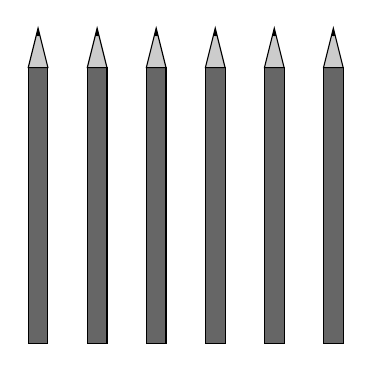
\begin{tikzpicture}
        \begin{scope}[scale=0.5]
          \stift{ 0mm}{0cm}{0}
          \stift{15mm}{0cm}{0}
          \stift{30mm}{0cm}{0}
          \stift{45mm}{0cm}{0}
          \stift{60mm}{0cm}{0}
          \stift{75mm}{0cm}{0}
        \end{scope}
      \end{tikzpicture}
    \end{center}
  \fi
  \ifoutline\outline
    Versuche zunächst \emph{drei} Stifte so zu legen, dass jeder
    jeden berührt\ldots
  \fi
  \ifoutcome\outcome
    Zuerst werden auf der unteren Ebene drei Stifte so gelegt,
    dass jeder jeden berührt. Dieses Schema wiederholt man dann
    einfach auf der zweiten Ebene.
    \begin{center}
      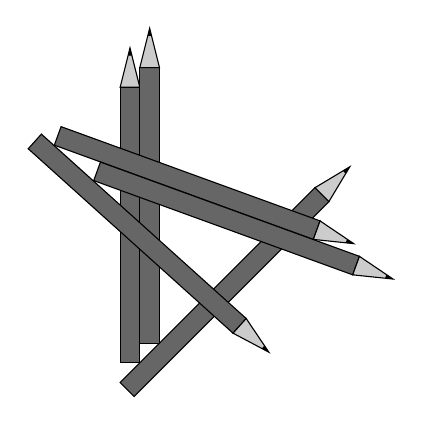
\begin{tikzpicture}
        \begin{scope}[scale=0.5]
          \stift{ 0.00cm}{ 0.00cm}{0}
          \stift{ 0.50cm}{ 0.50cm}{0}
          \stift{ 0.00cm}{-0.50cm}{315}
          \stift{-1.50cm}{ 6.00cm}{250}
          \stift{-0.50cm}{ 5.10cm}{250}
          \stift{-2.00cm}{ 5.81cm}{228}
        \end{scope}
      \end{tikzpicture}
    \end{center}
  \fi
\end{exercise}
